\documentclass[a4paper,10pt]{article}
\usepackage[dvips]{color,graphicx}
\usepackage[dvips, bookmarks, colorlinks=false]{hyperref}


%opening
\title{Math508 Homework 7}
\author{Yu Huang}

\begin{document}

\maketitle

\begin{abstract}
Viterbi Decoding Algorith to find optimal path
\end{abstract}

\section{No. 1}
Tossing of coins with initial coin randomly(uniformly) selected. Tossing continues possibly changing the coin with probability $1/3$. Assume we observed $Y_{[0,10]} = HHHHTHTTTT$.

The optimal path (order of coins chosen) found by Viterbi algorithm is 
\begin{verbatim}
[1, 1, 1, 1, 3, 1, 3, 3, 3, 3]
\end{verbatim}


\section{No. 2}
Hidden markov model on a simple reflected r.w. $X_n$ on A[0,20] starting at 10. $P(W_1 = \pm L) = \frac{1}{2}$. $Y_n = min\{max\{X_n+W_n, 0\}, 20\}$. Simulate $X_n$, $Y_n$, $0 \le n \le 400$, for $L=10,14,16,17$, find two optimal path estimates $X^{\ast max}_n$ and $X^{\ast min}_n$ of $X_n$ by choosing maximal and minimal solution of the maximization problem in every Viterbi Algorithm step.

For $L=10$, check Figure~\ref{f2}; for $L=14$, check Figure~\ref{f3}; for $L=16$, check Figure~\ref{f4}; for $L=17$, check Figure~\ref{f5}.

\begin{figure}[p]
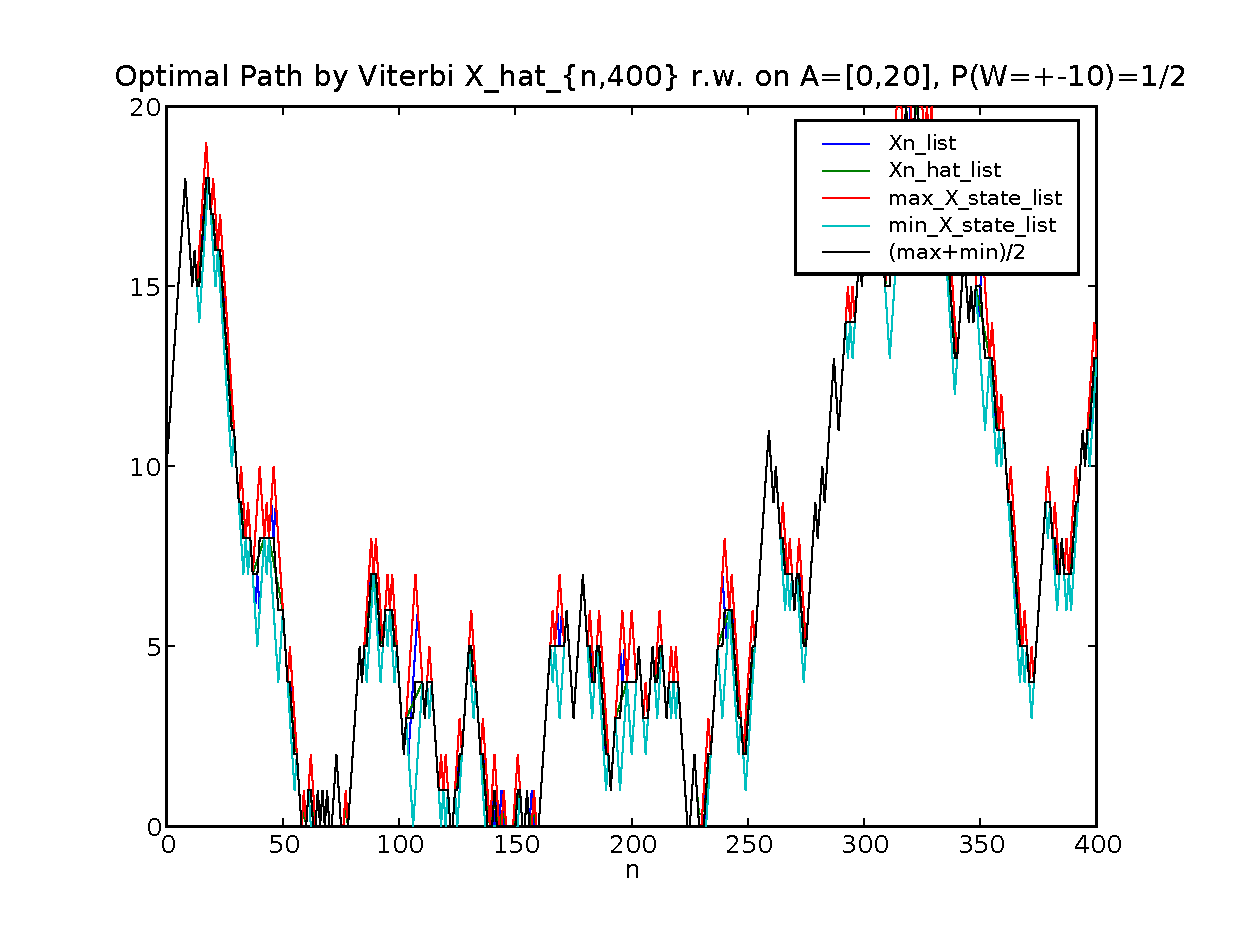
\includegraphics[width=1\textwidth]{hw7_2_K_20_L_10_T_400.eps}
\caption{}\label{f2}
\end{figure}

\begin{figure}[p]
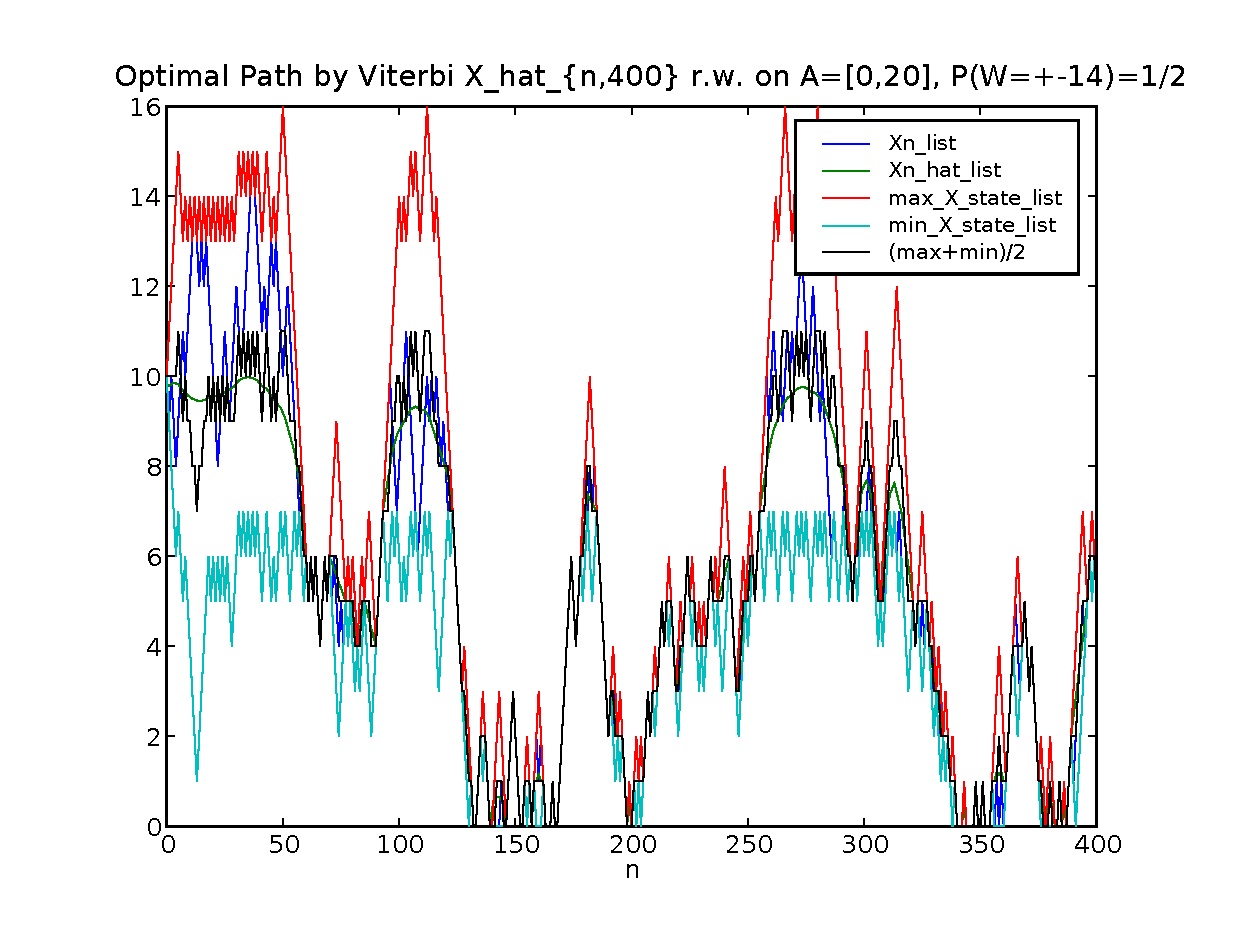
\includegraphics[width=1\textwidth]{hw7_2_K_20_L_14_T_400.eps}
\caption{}\label{f3}
\end{figure}

\begin{figure}
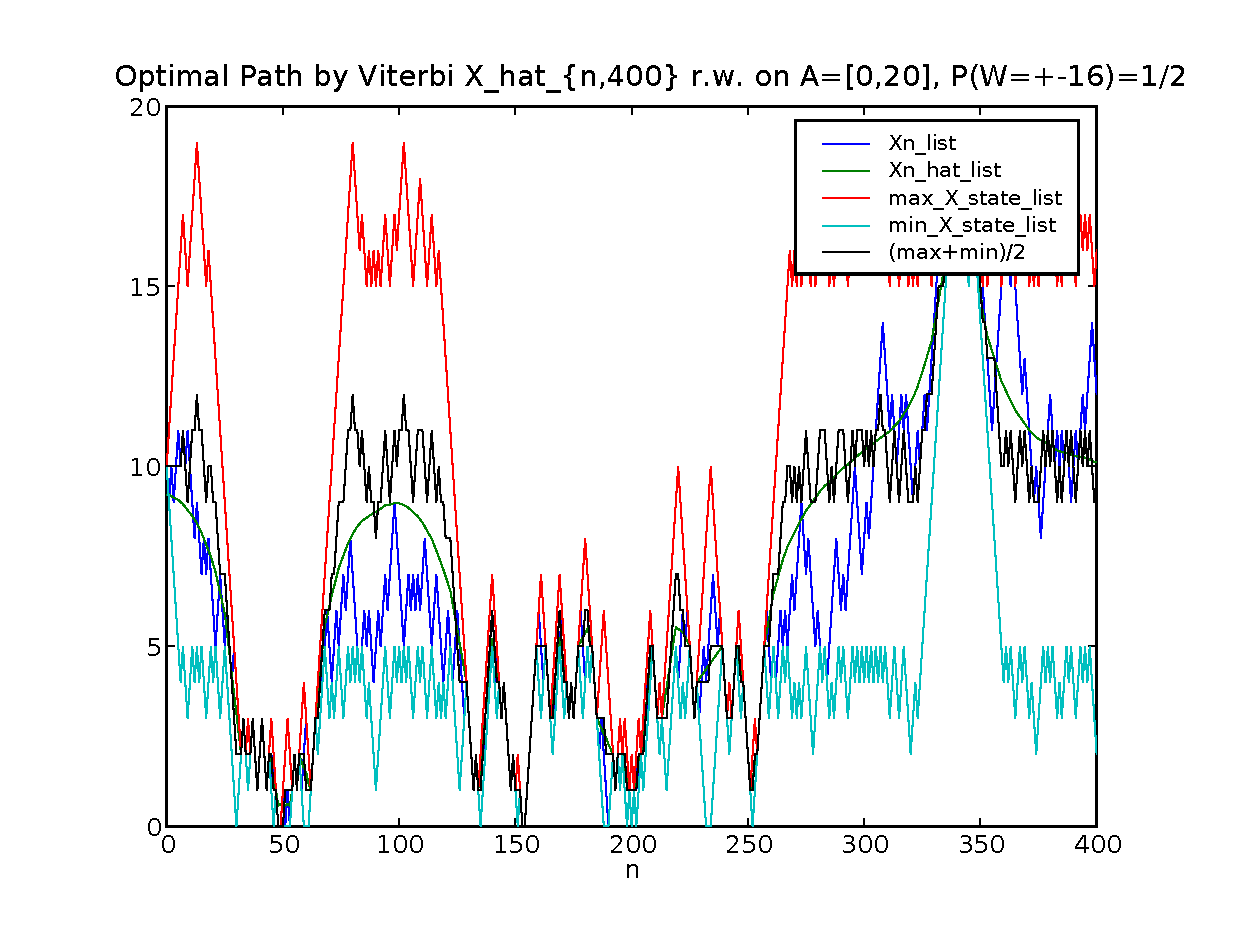
\includegraphics[width=1\textwidth]{hw7_2_K_20_L_16_T_400.eps}
\caption{}\label{f4}
\end{figure}

\begin{figure}
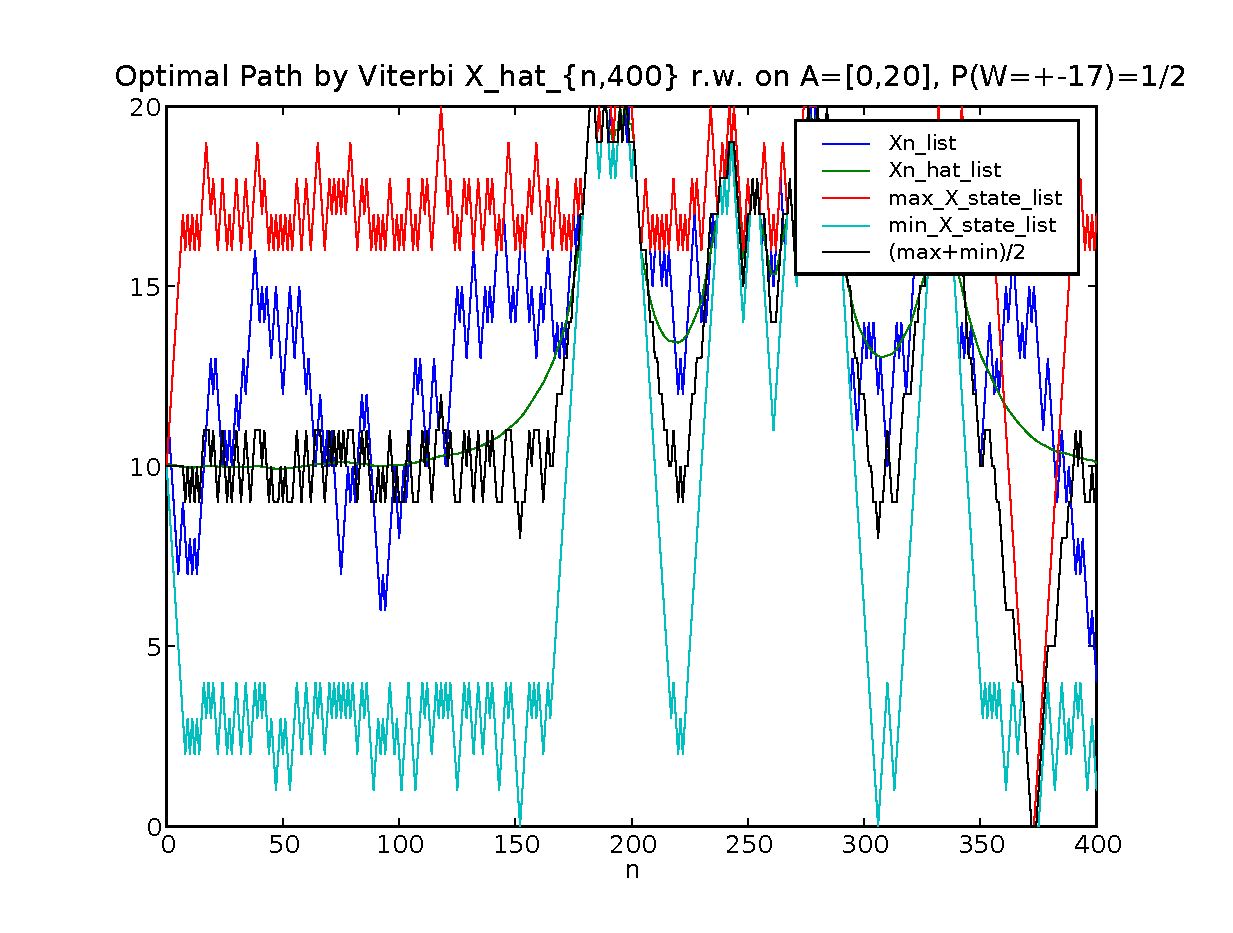
\includegraphics[width=1\textwidth]{hw7_2_K_20_L_17_T_400.eps}
\caption{}\label{f5}
\end{figure}

\end{document}
